\makeatletter % Use \makeatletter to make '@' a letter
\def\input@path{{../}} % Define input path to parent directory
\makeatother % Restore default category code of '@'

\documentclass[../Tesi_Jiahao_Miao_986136.tex]{subfiles}

\begin{document}

\section{Matching of resummation to fixed-order calculations}\label{sec:Matching}

Having obtained a resummed expression such as \cref{eq:RT_resummed} for the shape cross sections at small values
of $\tau$, one can now match the resummed expression to the fixed-order NNLO calculations at large values of $\tau$
using the R-matching scheme \cite{CATANI19933}. The results presented in the previous sections allow us to 
compare the predictions at N$^3$LL accuracy with the fixed-order calculations at NNLO.

In the R-matching scheme, at N$^3$LL+NNLO accuracy the matching procedure is given by:

\begin{flalign}\label{eq:R-matching}
    R_T(\tau) &= (1 + C_1 \bar{\alpha}_s+ C_2 \bar{\alpha}_s^2+ C_3 \bar{\alpha}_s^3) \exp{L g_1(\lambda)+ g_2(\lambda)+ \alpha_s g_3(\lambda)+\alpha_s^2 g_4(\lambda)}\\
    &+ D_1(\tau) \bar{\alpha}_s+ D_2(\tau) \bar{\alpha}_s^2+ D_3(\tau) \bar{\alpha}_s^3, \nonumber
\end{flalign}

where the coefficients $C_i$ are determined by imposing the normalization $R_T (\tau_{max}) = 1$ of the fixed order calculation order by order, while 
the remainder function $D_i$ are determined by subtracting from the fixed order terms $A,B$ and $C$ the logarithmic terms already present in \cref{eq:resummed_R}
(see \cref{eq:remainder function}).

$D_1$ is analytical \cite{CATANI19933}:

\begin{flalign}
    D_1(\tau) &= C_F \Bigl(-4 \text{Li}_2\left(\frac{t}{1-t}\right)+\frac{9 t^2}{2}-2 \ln ^2(1-t)+6 t (\ln (t)+1)\\
    &+4 \ln (1-t) \ln (t)+3 (1-2 t) \ln (1-2 t)\Bigr), \nonumber
\end{flalign}

while $D_2$ and $D_3$ are extracted numerically from interpolating the fixed order results at NNLO given in \cite{Weinzierl_2009}, the results are shown in \cref{fig:Fixed_order}.

By combining the resummed expression \cref{eq:resummed_R} and the fixed order results at NNLO, we can obtain the matched results at N$^3$LL+NNLO accuracy, we also reproduced the NLO+NLL \cite{CATANI19933,CATANI1991491} and NNLO+NNLL \cite{Monni:2011gb} accuracy already present in literature. 
The results are shown in \cref{fig:Matching}.

\begin{figure}
    \centering
    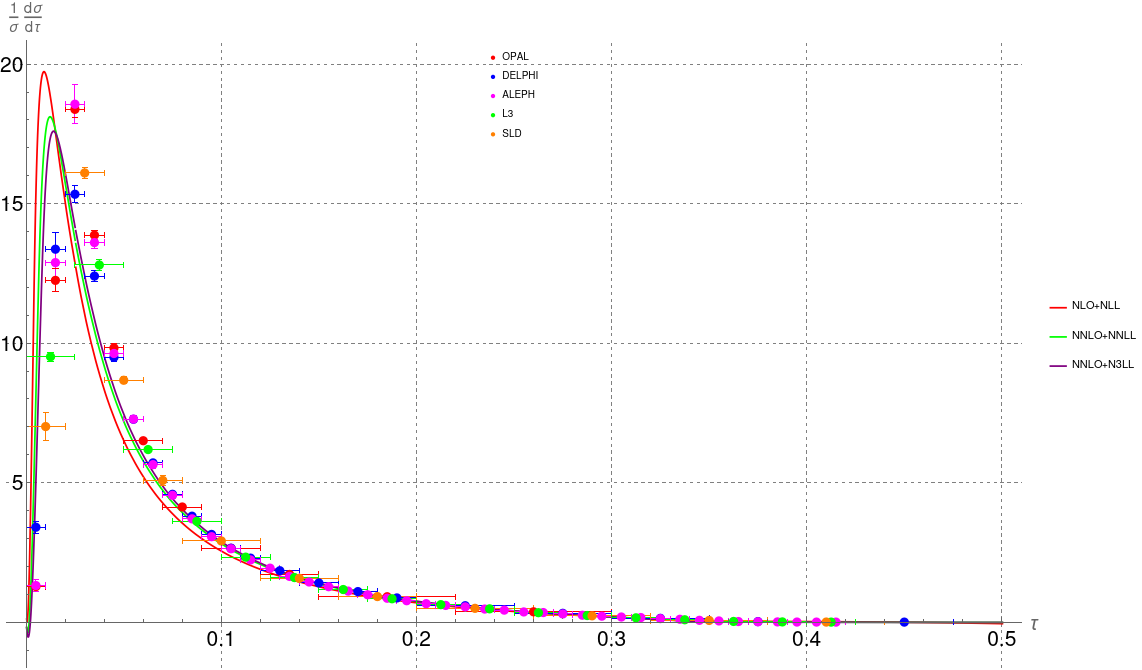
\includegraphics[width=0.8\textwidth]{figures/Matching.png}
    \caption{Plot of the matched Thrust distribution \cref{eq:R-matching} at NNLO+N$^3$LL accuracy.}
    \label{fig:Matching}
\end{figure}

\begin{figure}
    \centering
    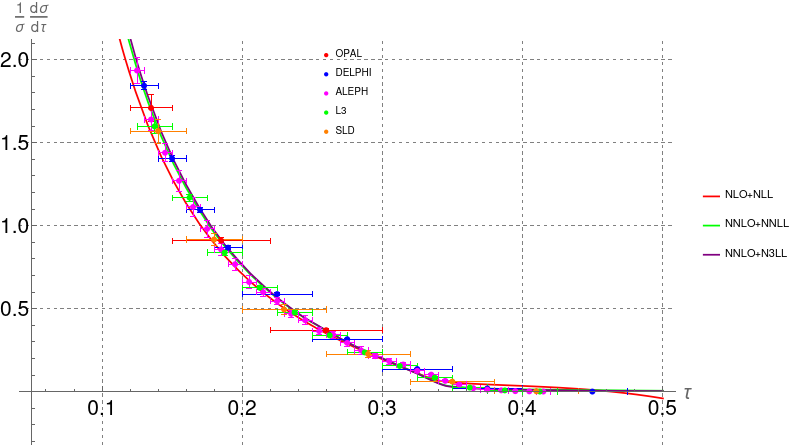
\includegraphics[width=0.8\textwidth]{figures/matched_tail_region.png}
    \caption{Plot of the matched Thrust distribution at NNLO+N$^3$LL and NNLO+NNLL accuracy in the tail region.}
\end{figure}

\begin{figure}
    \centering
    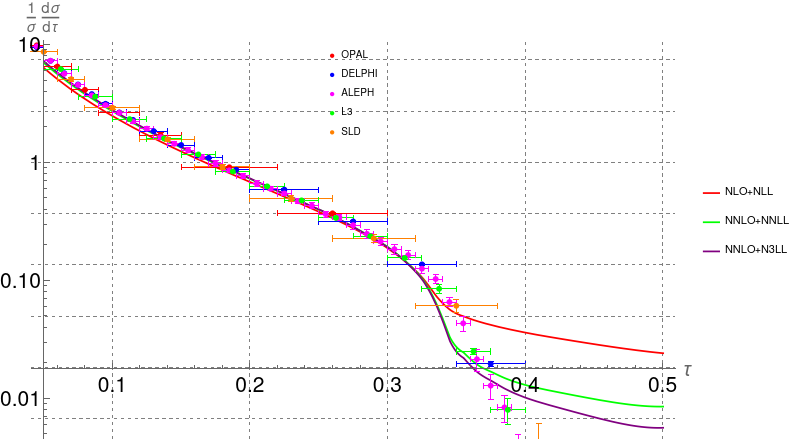
\includegraphics[width=0.8\textwidth]{figures/matched_tail_region_logplot.png}
    \caption{Log Plot of the matched Thrust distribution at NNLO+N$^3$LL and NNLO+NNLL accuracy in the tail region.}
\end{figure}

Resummation only slightly improves the fixed-order results at large values of $\tau$ as it includes some terms from higher
orders in the perturbative expansion \cref{eq:Fixed_order}, see \cref{tab:resummed vs fixed-order}.

\end{document}


% using the log(R)-matching scheme \cite{CATANI19933}. The results presented in the previous sections allow us to 
% compare the predictions at N$^3$LL accuracy with the fixed-order calculations at NNLO.

% In the log(R)-matching scheme, at N$^3$LL+NNLO accuracy the matching procedure is given by comparing 
% the logarithm of the fixed order result \cref{eq:Fixed_order}:

% \begin{equation}
%     \ln(R_T(\tau))= A(\tau) \bar{\alpha}_s + \qty( B(\tau) - \frac{1}{2}A^2(\tau)) \bar{\alpha}_s^2 + \qty(C(\tau) - A(\tau) B(\tau) + \frac{1}{3}A^3(\tau)) \bar{\alpha}_s^3 + \order{\bar{\alpha}_s^4}, 
% \end{equation}

% with the resummed expression \cref{eq:RT resummed} and subtracting the common logarithmic terms, one obtains the following expression:

% \begin{flalign}\label{eq:matching}
%         \ln(R(\tau,Q)) &= L g_1(\lambda)+ g_2(\lambda)+ \alpha_s g_3(\lambda)+\alpha_s^2 g_4(\lambda)\\
%         &+ \bar{\alpha}_s \qty( A(\tau) - G_{12}L^2 - G_{11}L) \nonumber\\
%         &+ \bar{\alpha}_s^2 \qty( B(\tau) - \frac{1}{2}A^2(\tau) -G_{23}L^3 - G_{22}L^2 - G_{21}L ) \nonumber\\
%         &+ \bar{\alpha}_s^3 \qty( C(\tau) - A(\tau) B(\tau) + \frac{1}{3}A^3(\tau) -G_{34}L^4 - G_{33}L^3 - G_{32}L^2 - G_{31}L )\nonumber
% \end{flalign}